% Four-pyramid P-ABCD: solid PA,PB,PC,AB,BC; dashed PD,DA,DB,DC.
% Coordinates in cm; schematic perspective projection, not metric.
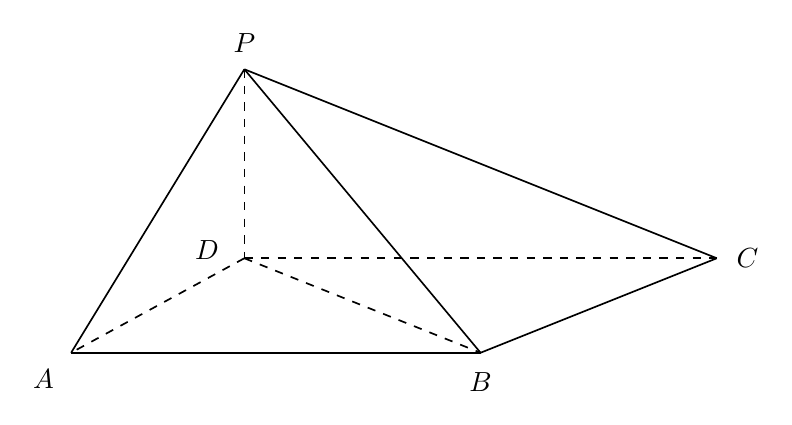
\begin{tikzpicture}[x=1cm,y=1cm,font=\normalsize,
  geometry edge/.style={draw=black,solid,line width=.6pt},
  geometry label/.style={font=\normalsize,inner sep=2pt}]
\coordinate (P) at (2.2,4.4);
\coordinate (D) at (2.2,2.0);
\coordinate (A) at (0,0.8);
\coordinate (B) at (5.2,0.8);
\coordinate (C) at (8.2,2.0);
% base front edges (visible)
\draw[geometry edge] (A)--(B);
\draw[geometry edge] (B)--(C);
% lateral visible edges
\draw[geometry edge] (P)--(A);
\draw[geometry edge] (P)--(B);
\draw[geometry edge] (P)--(C);
% hidden edges
\draw[geometry edge,dashed] (P)--(D);
\draw[geometry edge,dashed] (D)--(A);
\draw[geometry edge,dashed] (D)--(B);
\draw[geometry edge,dashed] (D)--(C);
% labels with clearance from strokes
\node[geometry label,above,yshift=4pt] at (P) {$P$};
\node[geometry label,left,xshift=-7pt,yshift=3pt] at (D) {$D$};
\node[geometry label,below left,xshift=-4pt,yshift=-4pt] at (A) {$A$};
\node[geometry label,below,yshift=-5pt] at (B) {$B$};
\node[geometry label,right,xshift=5pt] at (C) {$C$};
\end{tikzpicture}
